\documentclass[main.tex]{subfiles}
\begin{document}

\href{https://www2.seas.gwu.edu/~simhaweb/quantum/modules/module7/module7.html}{Module 7: Quantum circuits - universality}

\subsection{Universality: 1-qubit gates}

    We have seen several examples of building one gate from a combination of others. We now ask the question: can an arbitrary 1-qubit unitary operation be constructed from gates we've already constructed? Let
    
    $$
    U=\left[\begin{array}{ll}
    u_{00} & u_{01} \\
    u_{10} & u_{11}
    \end{array}\right]
    $$
    
    be an arbitrary unitary matrix with complex numbers $u_{00}, u_{01}, u_{10}, u_{11}$. We will show that one can find parameters $\alpha, \beta, \gamma, \delta$ such that
    
    $$
    U=K(\delta) T(\alpha) R(\beta) T(\gamma)
    $$
    
    That is reference Figure \ref{fig:01universal1}.
    
    \begin{figure}
        \centering
        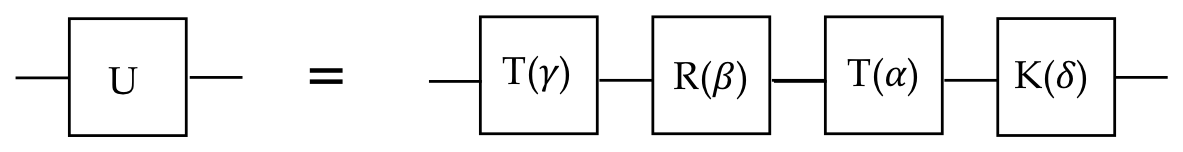
\includegraphics[width=4in]{notes/figs/n09/01universal1.png}
        \caption{unitary matrix parameters}
        \label{fig:01universal1}
    \end{figure}
    
    Recall:
    
    $$
    \begin{aligned}
    &T(\alpha)=e^{i \alpha Z}=\left[\begin{array}{cc}
    e^{i \alpha} & 0 \\
    0 & e^{-i \alpha}
    \end{array}\right] \\
    &R(\beta)=e^{i \beta Y}=\left[\begin{array}{cc}
    \cos \beta & \sin \beta \\
    -\sin \beta & \cos \beta
    \end{array}\right] \\
    &K(\delta)=e^{i \delta I}=\left[\begin{array}{cc}
    e^{i \delta} & 0 \\
    0 & e^{i \delta}
    \end{array}\right]
    \end{aligned}
    $$
    
    Let's work through the steps: Since $U$ is unitary, $U U^{\dagger}=I$:
    
    $$
    U U^{\dagger}=\left[\begin{array}{ll}
    u_{00} & u_{01} \\
    u_{10} & u_{11}
    \end{array}\right]\left[\begin{array}{ll}
    u_{00}^{*} & u_{10}^{*} \\
    u_{01}^{*} & u_{11}^{*}
    \end{array}\right]=\left[\begin{array}{ll}
    u_{00} u_{00}^{*}+u_{01} u_{01}^{*} & u_{00} u_{10}^{*}+u_{01} u_{11}^{*} \\
    u_{10} u_{00}^{*}+u_{11} u_{01}^{*} & u_{10} u_{10}^{*}+u_{11} u_{11}^{*}
    \end{array}\right]
    $$
    
    Equating this to $I$, we get four equations:
    
    $$
    \begin{array}{r}
    \left|u_{00}\right|^{2}+\left|u_{01}\right|^{2}=1 \\
    \left|u_{10}\right|^{2}+\left|u_{11}\right|^{2}=1 \\
    u_{00} u_{10}^{*}+u_{01} u_{11}^{*}=0 \\
    u_{10} u_{00}^{*}+u_{11} u_{01}^{*}=0
    \end{array}
    $$
    
    From the third:
    
    $$
    \Rightarrow \quad \begin{array}{lll}
    u_{00} u_{10}^{*} & = & -u_{01} u_{11}^{*} \\
    \Rightarrow \quad & \left|u_{00}\right|^{2}\left|u_{10}\right|^{2} & =\left|u_{01}\right|^{2}\left|u_{11}\right|^{2}
    \end{array}
    $$
    
    In this, substitute $\left|u_{01}\right|^{2}=1-\left|u_{00}\right|^{2}$ and $\left|u_{10}\right|^{2}=1-\left|u_{11}\right|^{2}$ from the first two of the set of four equations earlier. This results in $\left|u_{00}\right|^{2}=\left|u_{11}\right|^{2}$. A similar substitution in the fourth equation results in $\left|u_{01}\right|^{2}=\left|u_{10}\right|^{2}$. We conclude:
    
    $$
    \begin{aligned}
    &\left|u_{00}\right|=\left|u_{11}\right| \\
    &\left|u_{01}\right|=\left|u_{10}\right|
    \end{aligned}
    $$
    
    Now, from the first two of earlier set of four, each $\left|u_{i j}\right| \leq 1$. For any complex $z=r e^{i \theta}$ such that $|z| \leq 1$, we have $r \leq 1$. This means we can find some $\beta$ such that $r=\cos \beta$. Thus, we can write, for example:
    
    $$
    u_{00}=e^{i \theta_{00}} \cos \beta
    $$
    
    Then, because $\left|u_{00}\right|^{2}=\left|u_{11}\right|^{2}$
    
    $$
    u_{11}=e^{i \theta_{11}} \cos \beta
    $$
    
    for some $\theta_{11}$. Note: We can't conclude $\theta_{00}=\theta_{11}$ from $\left|u_{00}\right|=\left|u_{11}\right|$. We can choose whether to use $\cos \beta$ or $-\cos \beta$. Both work. Since $\left|u_{01}\right|^{2}=1-\left|u_{00}\right|^{2}$,
    
    $$
    \left|u_{01}\right|^{2}=1-\left|u_{00}\right|^{2}=1-\cos ^{2} \beta=\sin ^{2} \beta
    $$
    
    Thus, either $\sin \beta$ or $-\sin \beta$ could be used in writing
    
    $$
    u_{01}=e^{i \theta_{01}} \sin \beta
    $$
    
    Putting it all together, $U$ can be written as
    
    $$
    \left[\begin{array}{ll}
    u_{00} & u_{01} \\
    u_{10} & u_{11}
    \end{array}\right]=\left[\begin{array}{cc}
    e^{i \theta_{00}} \cos \beta & e^{i \theta_{01}} \sin \beta \\
    -e^{i \theta_{10}} \sin \beta & e^{i \theta_{11}} \cos \beta
    \end{array}\right]
    $$
    
    Now equate $U=K(\delta) T(\alpha) R(\beta) T(\gamma)$ :
    
    $$
    \left[\begin{array}{cc}
    e^{i \theta_{00}} \cos \beta & e^{i \theta_{01}} \sin \beta \\
    -e^{i \theta_{10}} \sin \beta & e^{i \theta_{11}} \cos \beta
    \end{array}\right]=\left[\begin{array}{cc}
    e^{i(\delta+\alpha+\gamma)} \cos \beta & e^{i(\delta+\alpha-\gamma)} \sin \beta \\
    -e^{i(\delta-\alpha+\gamma)} \sin \beta & e^{i(\delta-\alpha-\gamma)} \cos \beta
    \end{array}\right]
    $$
    
    This results in equations:
    
    $$
    \begin{aligned}
    &\delta+\alpha+\gamma=\theta_{00} \\
    &\delta+\alpha-\gamma=\theta_{01} \\
    &\delta-\alpha+\gamma=\theta_{10} \\
    &\delta-\alpha-\gamma=\theta_{11}
    \end{aligned}
    $$
    
    We have four equations in three variables, which looks over-constrained, but there is linear dependence: Only the first three are needed. To see why, consider the fourth of the original set of four equations in the elements of $U$ :
    
    $$
    u_{10} u_{00}^{*}+u_{11} u_{01}^{*}=0
    $$
    
    Substituting from the newly formed matrix, this gives
    
    $$
    -e^{i \theta_{10}} \sin \beta e^{-i \theta_{00}} \cos \beta+e^{i \theta_{11}} \cos \beta e^{-i \theta_{01}} \sin \beta=0
    $$
    
    From which
    
    $$
    e^{i\left(\theta_{11}-\theta_{01}\right)}=e^{i\left(\theta_{10}-\theta_{00}\right)}
    $$
    
    and thus
    
    $$
    \theta_{11}-\theta_{01}=\theta_{10}-\theta_{00}
    $$
    
    That is, one of the $\theta^{\prime}$ s can be expressed in terms of the other three. Thus, in solving the equations, we must use only three of them. The parameters $\alpha, \beta, \gamma, \delta$ can now be chosen to create any unitary operation. For example, with $\alpha=\gamma=0, \beta=\delta=\frac{\pi}{2}$,
    
    $$
    \left[\begin{array}{cc}
    e^{i(\delta+\alpha+\gamma)} \cos \beta & e^{i(\delta+\alpha-\gamma)} \sin \beta \\
    -e^{i(\delta-\alpha+\gamma)} \sin \beta & e^{i(\delta-\alpha-\gamma)} \cos \beta
    \end{array}\right]=\left[\begin{array}{cc}
    0 & e^{0} \sin \frac{\pi}{2} \\
    -e^{i \pi} \sin \frac{\pi}{2} & 0
    \end{array}\right]=\left[\begin{array}{ll}
    0 & 1 \\
    1 & 0
    \end{array}\right]=X
    $$
    
\subsection{Universality: controlled-U}

    Once a particularly useful unitary $U$ is found, one would like to turn it on or as needed. That is, design a Controlled-$U$ in terms of the same basic gates $K(\delta), T(\alpha), R(\beta)$ as shown in Figure \ref{fig:02universal2}.
    
    \begin{figure}
        \centering
        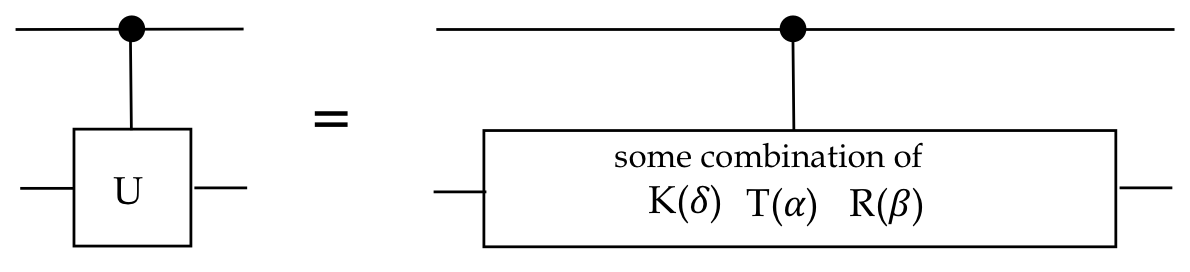
\includegraphics[width=4in]{notes/figs/n09/02universal2.png}
        \caption{Controlled - $U$}
        \label{fig:02universal2}
    \end{figure}
    
    Recall:
    
    $$
    \begin{aligned}
    K(\delta) &=e^{i \delta I}=\left[\begin{array}{cc}
    e^{i \delta} & 0 \\
    0 & e^{i \delta}
    \end{array}\right] \\
    T(\alpha) &=e^{i \alpha Z}=\left[\begin{array}{cc}
    e^{i \alpha} & 0 \\
    0 & e^{-i \alpha}
    \end{array}\right] \\
    R(\beta) &=e^{i \beta Y}=\left[\begin{array}{cc}
    \cos \beta & \sin \beta \\
    -\sin \beta & \cos \beta
    \end{array}\right]
    \end{aligned}
    $$
    
    We will also need at least one Controlled gate, for which we'll prefer to use $C_{NOT}$. Thus, the gate set we wish to use consists of: $C_{NOT}, K(\delta), T(\alpha), R(\beta)$. The starting point is a general $U$ in the form
    
    $$
    U=K(\delta) T(\alpha) R(\beta) T(\gamma)
    $$
    
    as shown in the previous section. First, we'll decompose Controlled-$U$ into two parts shown in Figure \ref{fig:03universal3}.

    \begin{figure}
        \centering
        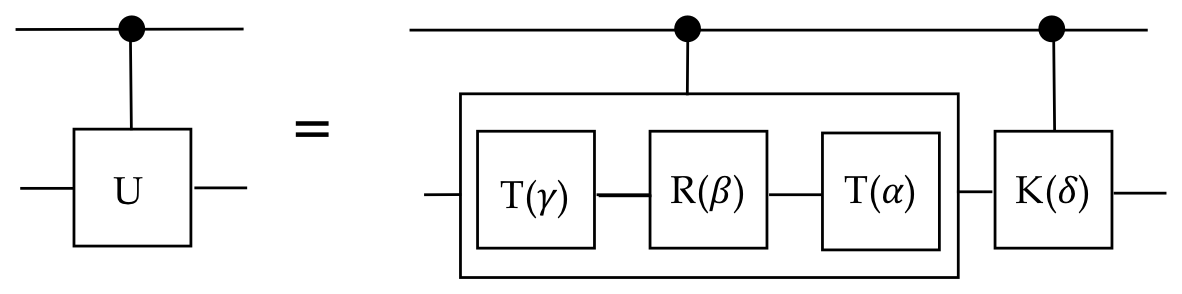
\includegraphics[width=4in]{notes/figs/n09/03universal3.png}
        \caption{Decompose Controlled-$U$}
        \label{fig:03universal3}
    \end{figure}
    
    What we seek is: With $|0\rangle$ as the control bit, neither unit is activated. With $|1\rangle$, both are, and the resulting unitary on the second qubit should be
    
    $$
    (K(\delta)) \quad(T(\alpha) R(\beta) T(\gamma))
    $$
    
    We now focus on the first part of the unitary product (last to act in the circuit) shown in Figure \ref{fig:04universal4}.
    
    \begin{figure}
        \centering
        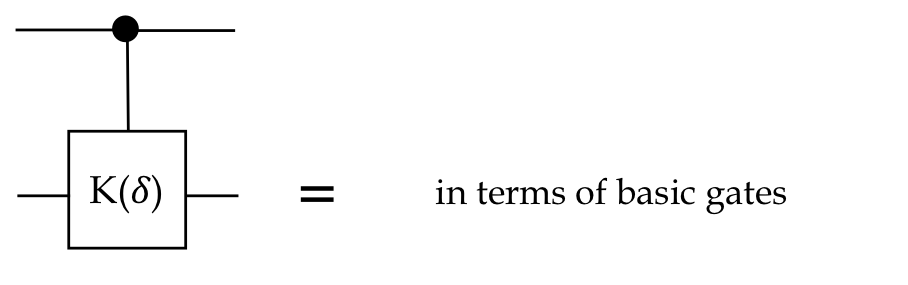
\includegraphics[width=4in]{notes/figs/n09/04universal4.png}
        \caption{first part of the unitary product}
        \label{fig:04universal4}
    \end{figure}
    
    Recall the Dirac version of $C_{NOT}$ :
    
    $$
    C_{NOT}=|0\rangle\langle 0|\otimes I+| 1\rangle\langle 1| \otimes X
    $$
    
    The intuition: When the control (first) qubit is $|0\rangle$, apply $I$ to the second qubit. When the control is $|1\rangle$, apply $X$. Then, Controlled- $K(\delta)$ can be written as:
    
    $$
    \text{Controlled}-K(\delta)=|0\rangle\langle 0|\otimes I+| 1\rangle\langle 1| \otimes K(\delta)
    $$
    
    Since $K(\delta)=e^{i \delta} I$
        
    $$
    \begin{aligned}
    &\text { Controlled }-K(\delta)=|0\rangle\langle 0|\otimes I+| 1\rangle\langle 1| \otimes K(\delta)\\
    &=|0\rangle\langle 0|\otimes I+| 1\rangle\langle 1| \otimes e^{i \delta} I \quad \text { Definition of } K(\delta)\\
    &=|0\rangle\left\langle 0\left|\otimes I+e^{i \delta}\right| 1\right\rangle\langle 1| \otimes I \quad \text { Bilinearity: constants can switch places in tensor }\\
    &=\left(|0\rangle\left\langle 0\left|+e^{i \delta}\right| 1\right\rangle\langle 1|\right) \otimes I \quad \text { Additivity of tensoring }
    \end{aligned}
    $$
    
    Recall: $\alpha|v\rangle \otimes|w\rangle=|v\rangle \otimes \alpha|w\rangle$. Continuing with the first term,
    
    $$
    \begin{aligned}
    |0\rangle\left\langle 0\left|+e^{i \delta}\right| 1\right\rangle\langle 1| &=\left[\begin{array}{ll}
    1 & 0 \\
    0 & 0
    \end{array}\right]+\left[\begin{array}{cc}
    0 & 0 \\
    0 & e^{i \delta}
    \end{array}\right] \\
    &=\left[\begin{array}{cc}
    e^{0} & 0 \\
    0 & e^{i \delta}
    \end{array}\right] \\
    &=\left[\begin{array}{cc}
    e^{-i \frac{\delta}{2}} e^{i \frac{\delta}{2}} & 0 \\
    0 & e^{i \frac{\delta}{2}} e^{i \frac{\delta}{2}}
    \end{array}\right] \\
    &=\left[\begin{array}{cc}
    e^{i \frac{\delta}{2}} & 0 \\
    0 & e^{i \frac{\delta}{2}}
    \end{array}\right]\left[\begin{array}{cc}
    e^{-i \frac{\delta}{2}} & 0 \\
    0 & e^{i \frac{\delta}{2}}
    \end{array}\right] \\
    &=K\left(\frac{\delta}{2}\right) T\left(-\frac{\delta}{2}\right)
    \end{aligned}
    $$
    
    Thus, substituting,
    
    $$
    \begin{aligned}
    \text { Controlled }-K(\delta) &=\left(|0\rangle\left\langle 0\left|+e^{i \delta}\right| 1\right\rangle\langle 1|\right) \otimes I \\
    &=K\left(\frac{\delta}{2}\right) T\left(-\frac{\delta}{2}\right) \otimes I
    \end{aligned}
    $$
    
    Note: the first part acts on the first qubit, and $I$ acts on the second. Let's draw this part of the circuit to see something surprising shown in Figure \ref{fig:05universal5}.
    
    \begin{figure}
        \centering
        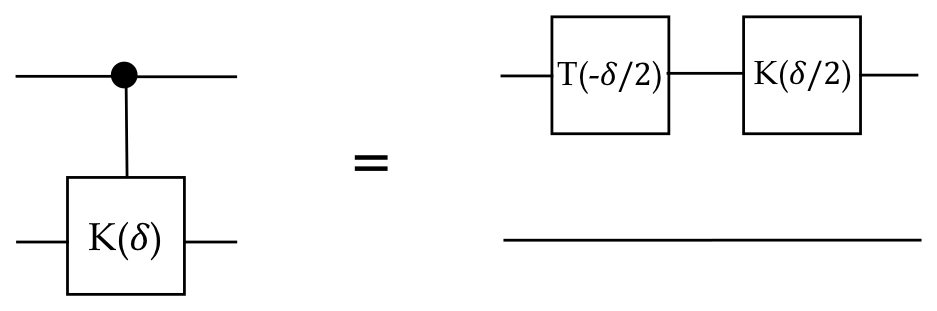
\includegraphics[width=4in]{notes/figs/n09/05universal5.png}
        \caption{$\text{Controlled}-K(\delta)$}
        \label{fig:05universal5}
    \end{figure}
    
    The second qubit, the one that is controlled, passes by untouched! This is an unusual case in that $K(\delta)=e^{i \delta} I$ is really multiplication by the constant $e^{i \delta}$. In a tensor, as we've seen, the constant can be moved between tensor terms. Thus, for example,
    
    $$
    A \otimes e^{i \delta} I=e^{i \delta} A \otimes I
    $$
    
    which makes it appear that the second qubit is untouched. What's important to realize is that the operation is on a 2 -qubit state, which can shuffle constants between its constituents. Next, let's turn to the second part of the overall decomposition shown in Figure \ref{fig:06universal6}.
    
    \begin{figure}
        \centering
        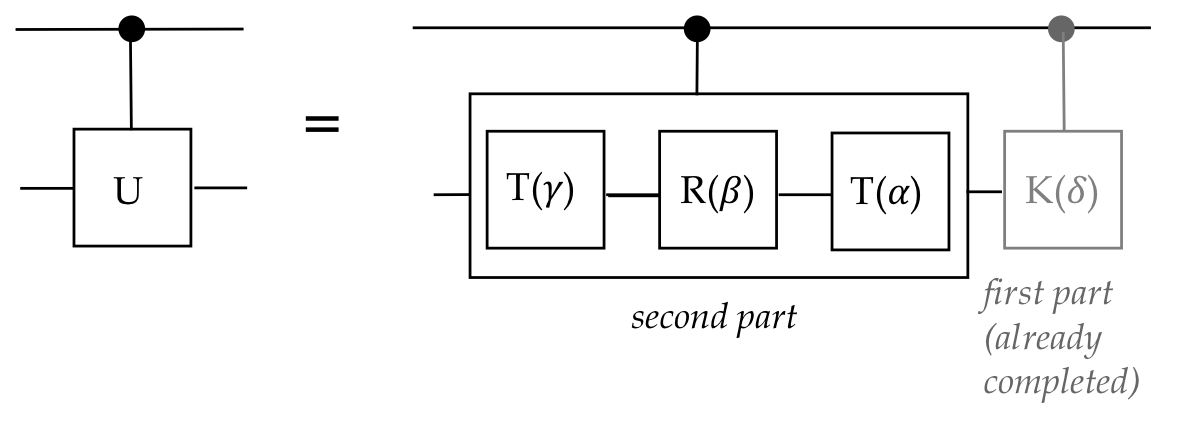
\includegraphics[width=4in]{notes/figs/n09/06universal6.png}
        \caption{Overall Decomposition}
        \label{fig:06universal6}
    \end{figure}
    
    The following results will be useful:
    
    $$
    \begin{aligned}
    T(0) &=I \\
    R(0) &=I \\
    T\left(\alpha_{1}+\alpha_{2}\right) &=T\left(\alpha_{1}\right) T\left(\alpha_{2}\right) \\
    R\left(\beta_{1}+\beta_{2}\right) &=T\left(\beta_{1}\right) T\left(\beta_{2}\right) \\
    X R(\beta) X &=R(-\beta) \\
    X T(\alpha) X &=T(-\alpha)
    \end{aligned}
    $$
    
    Next, let's work through the remaining steps: Define the following unitary combinations:
    
    $$
    \begin{aligned}
    U_{1} &=T(\alpha) R\left(\frac{\beta}{2}\right) \\
    U_{2} &=R\left(-\frac{\beta}{2}\right) T\left(-\frac{\gamma+\alpha}{2}\right) \\
    U_{3} &=T\left(\frac{\gamma-\alpha}{2}\right)
    \end{aligned}
    $$
    
    Then, the product of these is
    
    $$
    \begin{aligned}
    U_{1} U_{2} U_{3} &=T(\alpha) R\left(\frac{\beta}{2}\right) R\left(-\frac{\beta}{2}\right) T\left(-\frac{\gamma+\alpha}{2}\right) T\left(\frac{\gamma-\alpha}{2}\right) \\
    &=T(\alpha) R(0) T\left(-\frac{\gamma}{2}-\frac{\alpha}{2}\right) T\left(\frac{\gamma-\alpha}{2}\right) \\
    &=T(\alpha) T\left(-\frac{\gamma}{2}\right) T\left(-\frac{\alpha}{2}\right) T\left(\frac{\gamma}{2}\right) T\left(-\frac{\alpha}{2}\right) \\
    &=T\left(-\frac{\gamma}{2}\right) T\left(\frac{\gamma}{2}\right) T(\alpha) T\left(-\frac{\alpha}{2}\right) T\left(-\frac{\alpha}{2}\right) \\
    &=T(0) T(0) \\
    &=I
    \end{aligned}
    $$
    
    Now consider the product $U_{1} X U_{2} X U_{3}$, with $X$ interleaved:
    
    $$
    \begin{array}{rlr}
    U_{1} X U_{2} X U_{3} & =T(\alpha) R\left(\frac{\beta}{2}\right) X R\left(-\frac{\beta}{2}\right) T\left(-\frac{\gamma+\alpha}{2}\right), X T\left(\frac{\gamma-\alpha}{2}\right) & \text { Definitions of } U_{i} \\
    & =T(\alpha) R\left(\frac{\beta}{2}\right) X R\left(-\frac{\beta}{2}\right) X^{2} T\left(-\frac{\gamma+\alpha}{2}\right) X T\left(\frac{\gamma-\alpha}{2}\right) & X^{2}=I \\
    & =T(\alpha) R\left(\frac{\beta}{2}\right)\left(X R\left(-\frac{\beta}{2}\right) X\right)\left(X T\left(-\frac{\gamma+\alpha}{2}\right) X\right) T\left(\frac{\gamma-\alpha}{2}\right) & \text { Writing } X^{2}=X X \\
    & =T(\alpha) R\left(\frac{\beta}{2}\right)\left(R\left(\frac{\beta}{2}\right)\right)\left(T\left(\frac{\gamma+\alpha}{2}\right)\right) T\left(\frac{\gamma-\alpha}{2}\right) & \text { From exercise above } \\
    & =T(\alpha) R(\beta) T(\gamma) &
    \end{array}
    $$
    
    This is the second part of the overall decomposition. Let's summarize so far:
    
    $$
    \begin{aligned}
    U_{1} U_{2} U_{3} &=I \\
    U_{1} X U_{2} X U_{3} &=T(\alpha) R(\beta) T(\gamma)
    \end{aligned}
    $$
    
    Where each $U_{i}$ is constructed with basic gates $T(\alpha), R(\beta), K(\delta)$. Now consider the circuit shown in Figure \ref{fig:07universal7}.
    
    \begin{figure}
        \centering
        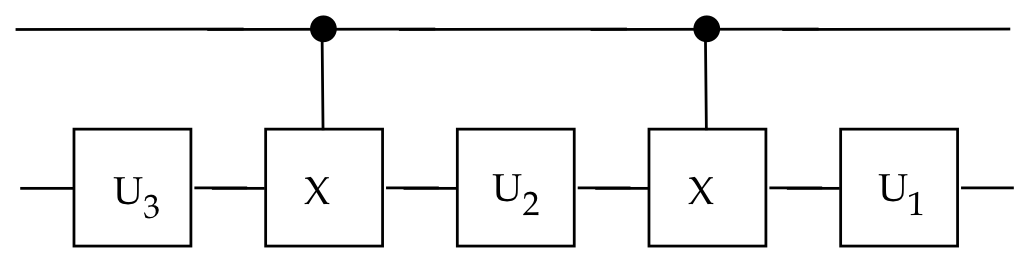
\includegraphics[width=4in]{notes/figs/n09/07universal7.png}
        \caption{$U_{1} X U_{2} X U_{3}$}
        \label{fig:07universal7}
    \end{figure}
    
    With the control qubit as $|0\rangle$ reference Figure \ref{fig:08universal8}.
    
    \begin{figure}
        \centering
        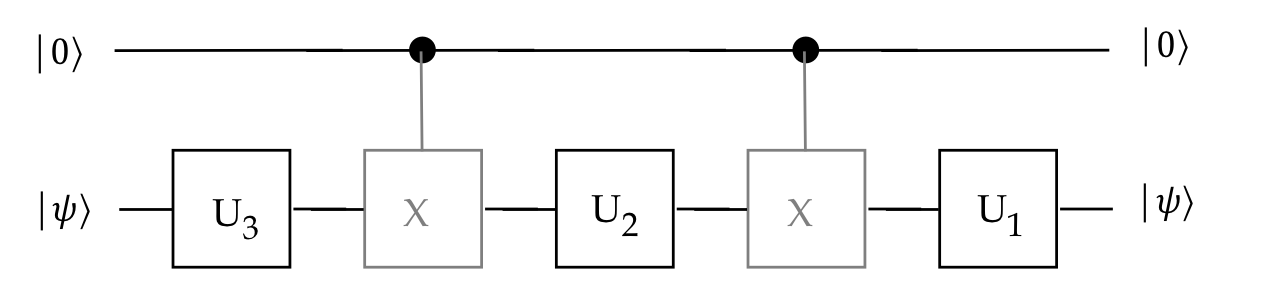
\includegraphics[width=4in]{notes/figs/n09/08universal8.png}
        \caption{$U_{1} X U_{2} X U_{3}$ with the control qubit as $|0\rangle$}
        \label{fig:08universal8}
    \end{figure}
    
    There's no change because we showed that $U_{1} U_{2} U_{3}=I$. With the control qubit as $|1\rangle$ shown in Figure \ref{fig:09universal9}.
    
    \begin{figure}
        \centering
        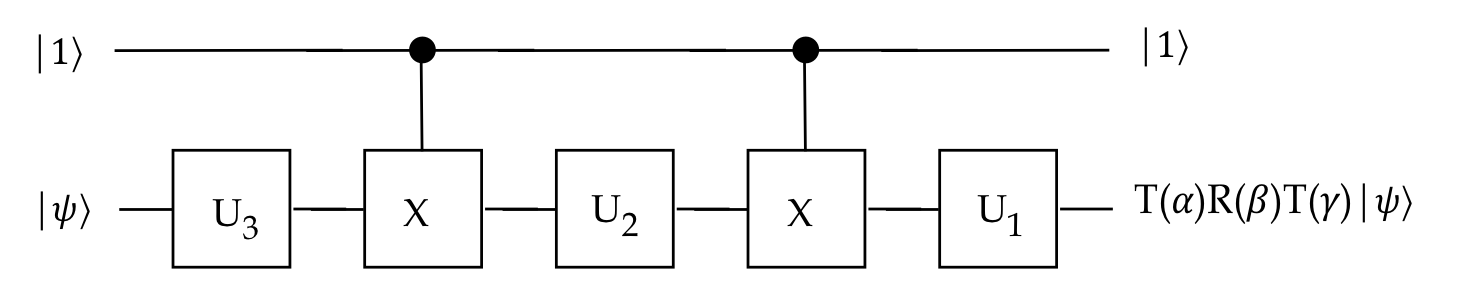
\includegraphics[width=4in]{notes/figs/n09/09universal9.png}
        \caption{$U_{1} X U_{2} X U_{3}$ with the control qubit as $|1\rangle$}
        \label{fig:09universal9}
    \end{figure}
    
    We obtain the second part of the overall decomposition: $U_{1} X U_{2} X U_{3}=T(\alpha) R(\beta) T(\gamma)$. Putting it all together in Figure \ref{fig:10universal10}.
    
    \begin{figure}
        \centering
        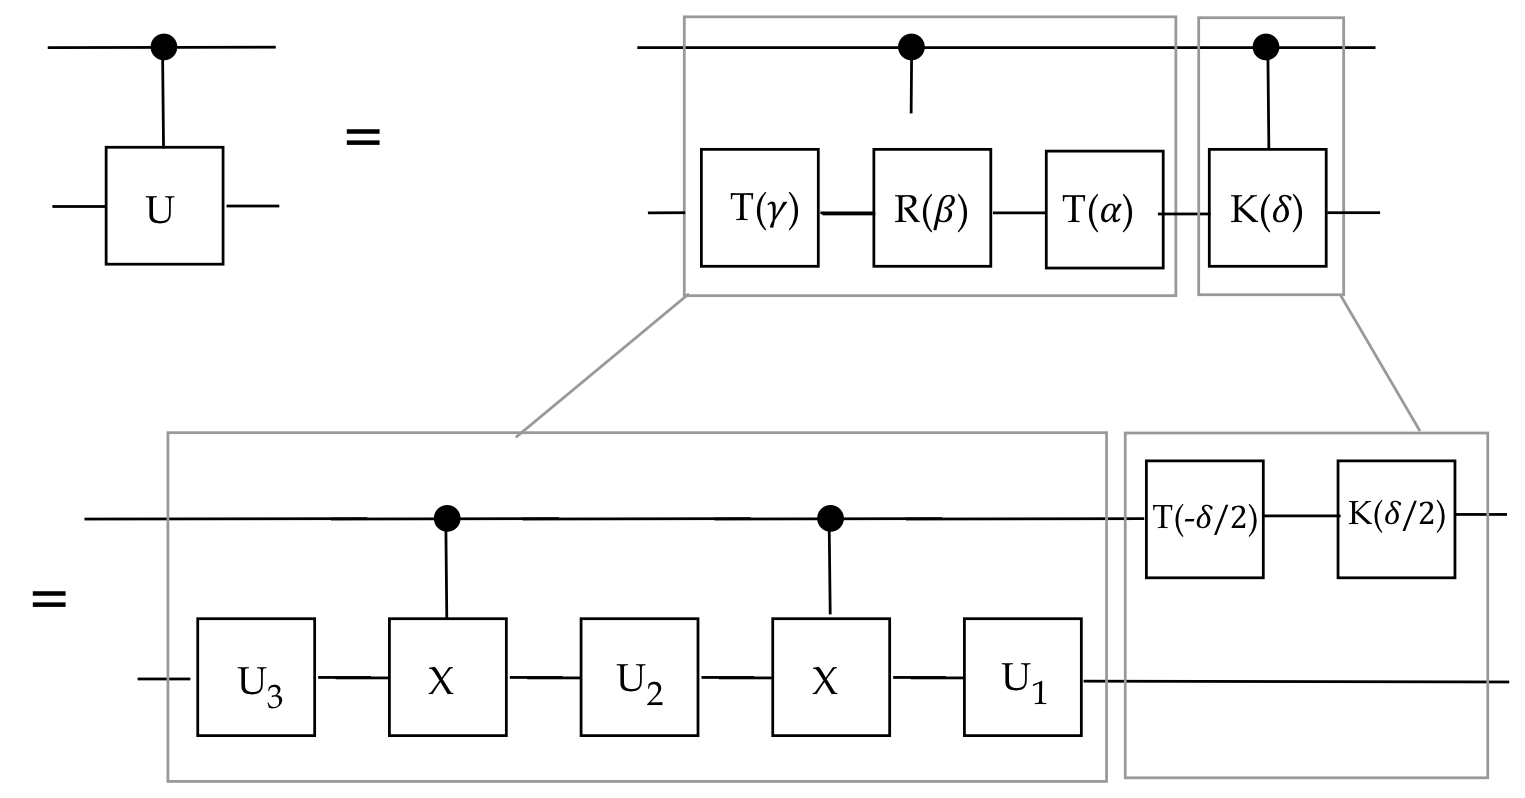
\includegraphics[width=4in]{notes/figs/n09/10universal10.png}
        \caption{Unitary all together}
        \label{fig:10universal10}
    \end{figure}
    
    Thus, we have a way to use basic gates to build any Controlled-$U$ gate.

\subsection{Controlled-controlled-U}

    The previous section showed how a singly-controlled $U$ can be expressed in terms of basic gates. In this section we consider doubly-controlled unitaries. Because a unitary $U$ is expressible as $V^{2}=U$ where $V$ is unitary then the 3-qubit Controlled-controlled-$U$ can be computed using only 2-qubit gates shown in Figure \ref{fig:11ccu}.
    
    \begin{figure}
        \centering
        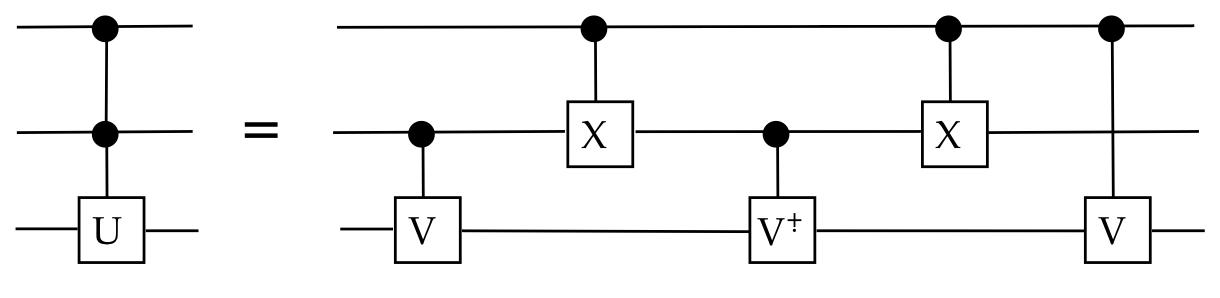
\includegraphics[width=4in]{notes/figs/n09/11ccu.png}
        \caption{3-qubit Controlled-controlled-$U$}
        \label{fig:11ccu}
    \end{figure}
    
    Here, $V^{2}=U$ and $V^{\dagger}=V^{-1}$. Let's consider the four cases for the top two qubits: $|00\rangle,|01\rangle,|10\rangle,|11\rangle$. Case: $|00\rangle$ is shown in Figure \ref{fig:12ccu2}.
    
    \begin{figure}
        \centering
        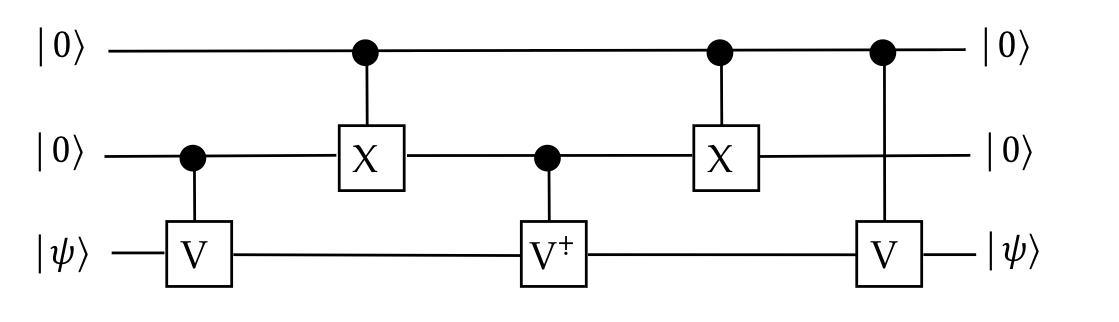
\includegraphics[width=4in]{notes/figs/n09/12ccu2.png}
        \caption{Case: $|00\rangle$}
        \label{fig:12ccu2}
    \end{figure}
    
    Here, none of the gates will be active, so the 3rd qubit is unchanged. Case: $|01\rangle$ is shown in Figure \ref{fig:13ccu3}.
    
    \begin{figure}
        \centering
        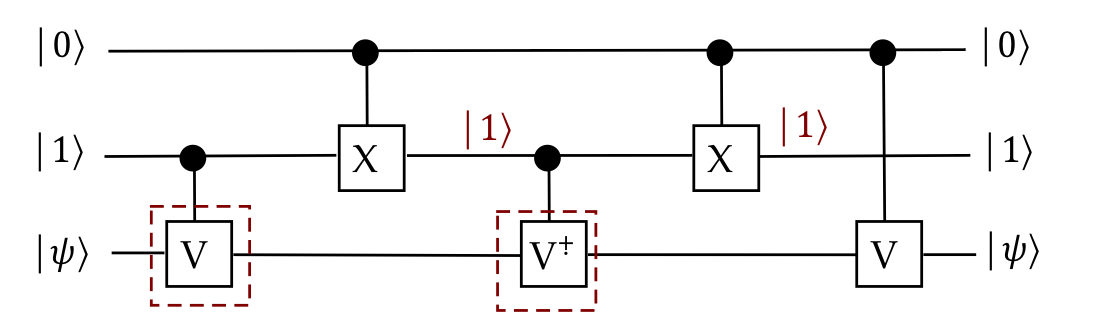
\includegraphics[width=4in]{notes/figs/n09/13ccu3.png}
        \caption{Case: $|01\rangle$}
        \label{fig:13ccu3}
    \end{figure}
    
    Now the active gates for the 3rd qubit result in
    
    $$
    V^{\dagger} V|\psi\rangle=|\psi\rangle
    $$
    
    Thus, no change. Case: $|10\rangle$ shown in Figure \ref{fig:14ccu4}.
    
    \begin{figure}
        \centering
        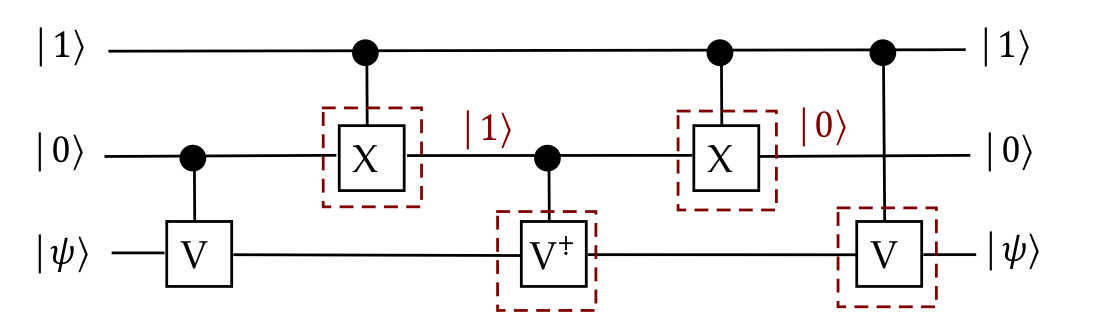
\includegraphics[width=4in]{notes/figs/n09/14ccu4.png}
        \caption{Case: $|10\rangle$}
        \label{fig:14ccu4}
    \end{figure}

    This time, the active gates for the 3rd qubit result in:
    
    $$
    V V^{\dagger}|\psi\rangle=|\psi\rangle
    $$

    Case: $|11\rangle$ shown in Figure \ref{fig:15ccu5}.
    
    \begin{figure}
        \centering
        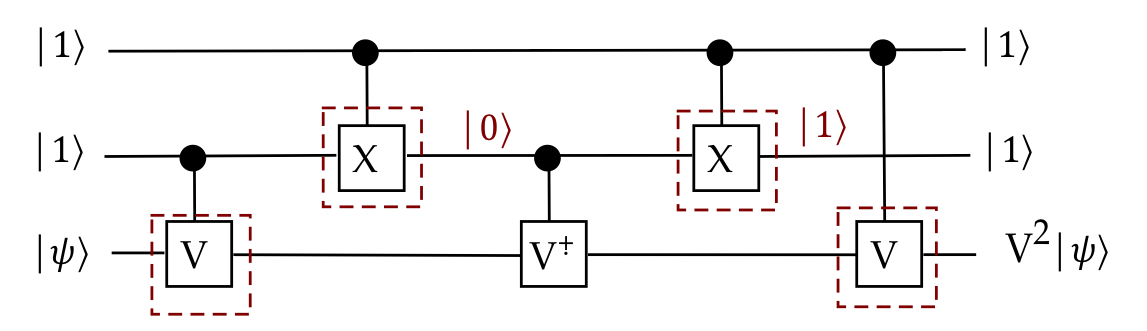
\includegraphics[width=4in]{notes/figs/n09/15ccu5.png}
        \caption{Case: $|11\rangle$}
        \label{fig:15ccu5}
    \end{figure}
    
    Now we see that
    
    $$
    V^{2}|\psi\rangle=U|\psi\rangle
    $$
    
    as desired. Of course, for arbitrary $U$, it may not be easy to find $V$ such that $V^{2}=U$: For matrices that can be easily exponentiated, we have seen how to do this. How can $V$ be computed? The spectral theorem that proves the existence of orthonormal eigenvectors applies to a broader class of matrices than Hermitians: the so-called normal matrices: $A$ is normal if $A A^{\dagger}=A^{\dagger} A$. Clearly, if $A$ is Hermitian $\left(A=A^{\dagger}\right)$, then $A$ is normal. So are unitaries because, by definition, $A=A^{\dagger}$. Apply the spectral theorem to write $U$ as
    
    $$
    U=S D S^{\dagger}
    $$
    
    where
    
    $$
    D=\text { Diagonal matrix with eigenvalues } \lambda_{i} \text { diagonal }
    $$
    
    $$
    S=\text { eigenvectors as columns }
    $$
    
    Let $D^{\frac{1}{2}}$ be the matrix with $\sqrt{\lambda_{i}}$ on the diagonal, and zeroes elsewhere. Then,
    
    $$
    \left(D^{\frac{1}{2}}\right)^{2}=D
    $$
    
    Now define
    
    $$
    V=S D^{\frac{1}{2}} S^{\dagger}
    $$
    
    Then
    
    $$
    V^{2}=\left(S D^{\frac{1}{2}} S^{\dagger}\right)\left(S D^{\frac{1}{2}} S^{\dagger}\right)=S D^{\frac{1}{2}}\left(S S^{\dagger}\right) D^{\frac{1}{2}} S^{\dagger}=U
    $$
    
    When computing $\sqrt{\lambda_{i}}$, there are two roots, and thus any choice of roots will result in one particular solution to $V^{2}=U$.

\subsection{Universality: multiply-controlled U}

    With the help of additional "spare" qubits, one can implement a multiply-controlled unitary in terms of doubly-controlled ones. Consider the following 4-controlled $U$ shown in Figure \ref{fig:16multicontrol}.
    
    \begin{figure}
        \centering
        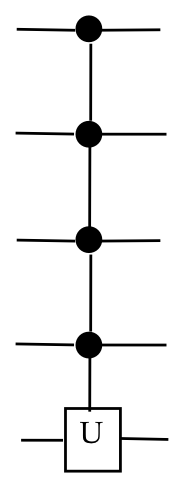
\includegraphics[width=1in]{notes/figs/n09/16multicontrol.png}
        \caption{4-controlled $U$}
        \label{fig:16multicontrol}
    \end{figure}
    
    We can use three additional qubits to achieve the same result with $CC_{NOT}$ gates and a doubly-controlled $U$ shown in Figure \ref{fig:17multicontrol2}.
    
    \begin{figure}
        \centering
        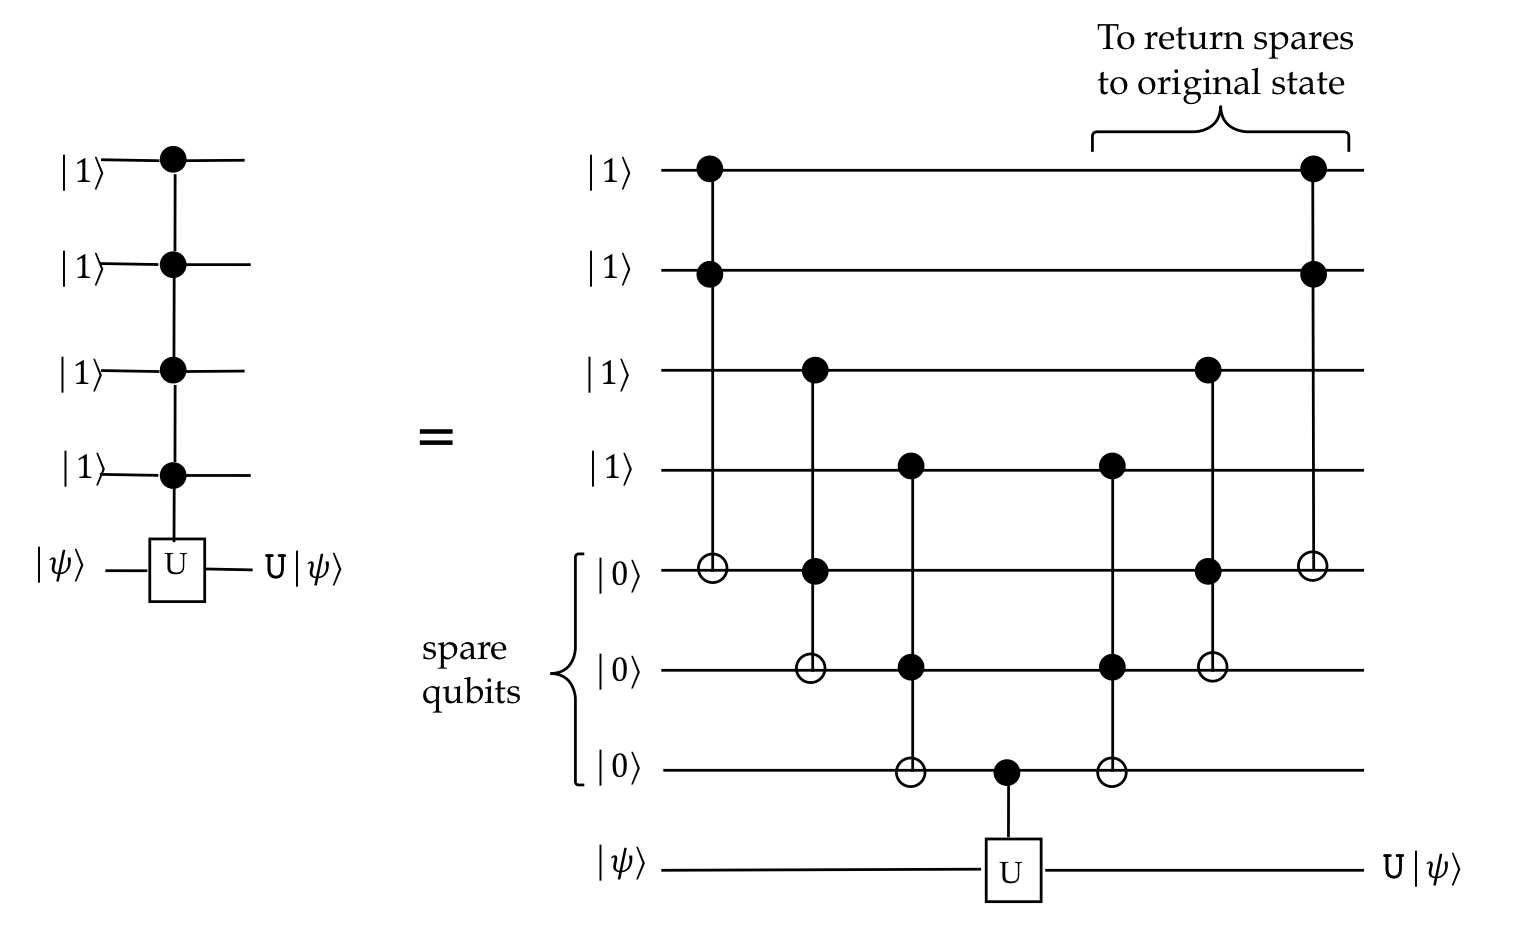
\includegraphics[width=5in]{notes/figs/n09/17multicontrol2.png}
        \caption{$CC_{NOT}$ gates and a doubly-controlled $U$}
        \label{fig:17multicontrol2}
    \end{figure}
    
    Clearly, any control-pattern can be accommodate by using the appropriate $CC_{NOT}$ gates (filled or unfilled circles).

\subsection{Universality: multi-qubit gates}

    We will now show that an arbitrary n-qubit unitary operation can be decomposed into multiply-controlled single-qubit operations. This means that, using the previous sections, any arbitrary n-qubit unitary can be implemented with controlled- $U$ 's and $C_{N O T}$ gates. The construction is fairly involved, so let's do this in steps. Step 1: A two-level unitary affects only two entries in a vector: Consider this modification of the 3-qubit identity:
    
    $$
    \left[\begin{array}{llllllll}
    1 & 0 & 0 & 0 & 0 & 0 & 0 & 0 \\
    0 & \mathbf{a} & 0 & 0 & 0 & 0 & 0 & 0 \\
    0 & 0 & 1 & 0 & 0 & 0 & 0 & 0 \\
    0 & 0 & 0 & 1 & 0 & 0 & 0 & 0 \\
    0 & 0 & 0 & 0 & 1 & 0 & 0 & 0 \\
    0 & 0 & 0 & 0 & 0 & 1 & 0 & 0 \\
    0 & 0 & 0 & 0 & 0 & 0 & \mathbf{d} & 0 \\
    0 & 0 & 0 & 0 & 0 & 0 & 0 & 1
    \end{array}\right]
    $$
    
    We've replaced two of the 1's along the diagonal with complex numbers $a$ and $d$. If we want the resulting matrix to be unitary, we will need to satisfy unit-length (rows and columns), and pairwise orthogonality amongst rows and columns. Accordingly, with minimal additional entries, let's add
    
    $$
    \left[\begin{array}{llllllll}
    1 & 0 & 0 & 0 & 0 & 0 & 0 & 0 \\
    0 & \mathbf{a} & 0 & 0 & 0 & 0 & \mathbf{b} & 0 \\
    0 & 0 & 1 & 0 & 0 & 0 & 0 & 0 \\
    0 & 0 & 0 & 1 & 0 & 0 & 0 & 0 \\
    0 & 0 & 0 & 0 & 1 & 0 & 0 & 0 \\
    0 & 0 & 0 & 0 & 0 & 1 & 0 & 0 \\
    0 & \mathbf{c} & 0 & 0 & 0 & 0 & \mathbf{d} & 0 \\
    0 & 0 & 0 & 0 & 0 & 0 & 0 & 1
    \end{array}\right]
    $$
    
    One can impose the unitarity conditions and obtain relationships between these numbers, such as: $|a|^{2}+|b|^{2}=1$. One possible solution is:
    
    $$
    \left[\begin{array}{cccccccc}
    1 & 0 & 0 & 0 & 0 & 0 & 0 & 0 \\
    0 & \mathbf{a} & 0 & 0 & 0 & 0 & \mathbf{c}^{*} & 0 \\
    0 & 0 & 1 & 0 & 0 & 0 & 0 & 0 \\
    0 & 0 & 0 & 1 & 0 & 0 & 0 & 0 \\
    0 & 0 & 0 & 0 & 1 & 0 & 0 & 0 \\
    0 & 0 & 0 & 0 & 0 & 1 & 0 & 0 \\
    0 & \mathbf{c} & 0 & 0 & 0 & 0 & -\mathbf{a}^{*} & 0 \\
    0 & 0 & 0 & 0 & 0 & 0 & 0 & 1
    \end{array}\right]
    $$
    
    where $a$ and $c$ satisfy $|a|^{2}+|c|^{2}=1$. Next, observe the action of such a matrix on a generic 3 -qubit vector:
    
    $$
    \left[\begin{array}{llllllll}
    1 & 0 & 0 & 0 & 0 & 0 & 0 & 0 \\
    0 & \mathbf{a} & 0 & 0 & 0 & 0 & \mathbf{b} & 0 \\
    0 & 0 & 1 & 0 & 0 & 0 & 0 & 0 \\
    0 & 0 & 0 & 1 & 0 & 0 & 0 & 0 \\
    0 & 0 & 0 & 0 & 1 & 0 & 0 & 0 \\
    0 & 0 & 0 & 0 & 0 & 1 & 0 & 0 \\
    0 & \mathbf{c} & 0 & 0 & 0 & 0 & \mathbf{d} & 0 \\
    0 & 0 & 0 & 0 & 0 & 0 & 0 & 1
    \end{array}\right]\left[\begin{array}{c}
    \alpha_{0} \\
    \alpha_{1} \\
    \alpha_{2} \\
    \alpha_{3} \\
    \alpha_{4} \\
    \alpha_{5} \\
    \alpha_{6} \\
    \alpha_{7}
    \end{array}\right]=\left[\begin{array}{c}
    \alpha_{0} \\
    \mathbf{a} \alpha_{1}+\mathbf{b} \alpha_{6} \\
    \alpha_{2} \\
    \alpha_{3} \\
    \alpha_{4} \\
    \alpha_{5} \\
    \mathbf{c} \alpha_{1}+\mathbf{d} \alpha_{6} \\
    \alpha_{7}
    \end{array}\right]
    $$
    
    Notice: only two entries in the vector are modified.
    
    In Dirac notation, the result is:
    
    $$
    \alpha_{0}|000\rangle+\left(\mathbf{a} \alpha_{1}+\mathbf{b} \alpha_{\mathbf{6}}\right)|\mathbf{0 0 1}\rangle \alpha_{2}|010\rangle+\alpha_{3}|011\rangle+\alpha_{4}|100\rangle+\alpha_{5}|101\rangle+\left(\mathbf{c} \alpha_{1}+\mathbf{d} \alpha_{6}\right)|\mathbf{1 1 0}\rangle+\alpha_{7}|111\rangle
    $$
    
    This corresponds to the two columns for $|001\rangle$ and $|110\rangle$. Thus, another way of saying "two entries are modified" is: the coefficients of two standard-basis vectors are modified. In general, for n-qubits: The resulting $2^{n} \times 2^{n}$ matrix will have two columns in which the four numbers lie. These columns will correspond to the two standard-basis vectors that get modified. We will call such a matrix a two-level unitary matrix. Note: the adjoint of a two-level unitary is a two-level unitary.
    
    $$
    \left[\begin{array}{cccccccc}
    1 & 0 & 0 & 0 & 0 & 0 & 0 & 0 \\
    0 & \mathbf{a} & 0 & 0 & 0 & 0 & \mathbf{c}^{*} & 0 \\
    0 & 0 & 1 & 0 & 0 & 0 & 0 & 0 \\
    0 & 0 & 0 & 1 & 0 & 0 & 0 & 0 \\
    0 & 0 & 0 & 0 & 1 & 0 & 0 & 0 \\
    0 & 0 & 0 & 0 & 0 & 1 & 0 & 0 \\
    0 & \mathbf{c} & 0 & 0 & 0 & 0 & -\mathbf{a}^{*} & 0 \\
    0 & 0 & 0 & 0 & 0 & 0 & 0 & 1
    \end{array}\right]^{\dagger}=\left[\begin{array}{cccccccc}
    1 & 0 & 0 & 0 & 0 & 0 & 0 & 0 \\
    0 & \mathbf{a}^{*} & 0 & 0 & 0 & 0 & \mathbf{c}^{*} & 0 \\
    0 & 0 & 1 & 0 & 0 & 0 & 0 & 0 \\
    0 & 0 & 0 & 1 & 0 & 0 & 0 & 0 \\
    0 & 0 & 0 & 0 & 1 & 0 & 0 & 0 \\
    0 & 0 & 0 & 0 & 0 & 1 & 0 & 0 \\
    0 & \mathbf{c} & 0 & 0 & 0 & 0 & -\mathbf{a} & 0 \\
    0 & 0 & 0 & 0 & 0 & 0 & 0 & 1
    \end{array}\right]
    $$
    
    Step 2: Any unitary can be expressed as a product of two-level unitaries: We'll use a 2-qubit example to explain how. Consider
    
    $$
    U=\left[\begin{array}{llll}
    u_{00} & u_{01} & u_{02} & u_{03} \\
    u_{10} & u_{11} & u_{12} & u_{13} \\
    u_{20} & u_{21} & u_{22} & u_{23} \\
    u_{30} & u_{31} & u_{32} & u_{33}
    \end{array}\right]
    $$
    
    We'll now apply a series of matrix multiplications to convert $U$ into the identity. Recall from row-reduced matrices in solving equations: we want to make the entries below $u_{00}$ all 0. We want to multiply $U$ by a matrix $U_{1}$ to make the entry below $u_{00}$ zero:
    
    $$
    U_{1} U=\left[\begin{array}{cccc}
    u_{00} & u_{01} & u_{02} & u_{03} \\
    \mathbf{0} & u_{11} & u_{12} & u_{13} \\
    u_{20} & u_{21} & u_{22} & u_{23} \\
    u_{30} & u_{31} & u_{32} & u_{33}
    \end{array}\right]
    $$
    
    Clearly, the second row of $U_{1}$ produces that number, and so
    
    $$
    U_{1}=\left[\begin{array}{cccc}
    1 & 0 & 0 & 0 \\
    u_{10} & -u_{00} & 0 & 0 \\
    0 & 0 & 1 & 0 \\
    0 & 0 & 0 & 1
    \end{array}\right]
    $$
    
    achieves the result. But $U_{1}$ is not unitary. To fix this, we adjust the "two-level" entries as we did with two-level unitaries so that
    
    $$
    U_{1}=\left[\begin{array}{cccc}
    \frac{u_{00}^{*}}{r_{1}} & \frac{u_{i 0}}{r_{1}} & 0 & 0 \\
    \frac{u_{1}}{r_{1}} & -\frac{u_{00}}{r_{1}} & 0 & 0 \\
    0 & 0 & 1 & 0 \\
    0 & 0 & 0 & 1
    \end{array}\right]
    $$
    
    where $\left|u_{00}\right|^{2}+\left|u_{10}\right|^{2}=r_{1}^{2}$ is both unitary and two-level (which will play a later role). Multiplication by $U_{1}$ will produce some result we'll call $B$ :
    
    $$
    U_{1} U=\left[\begin{array}{cccc}
    \frac{u_{00}^{*}}{r_{1}} & \frac{u_{0}^{*}}{r_{1}} & 0 & 0 \\
    \frac{u_{10}}{r_{1}} & -\frac{u_{00}}{r_{1}} & 0 & 0 \\
    0 & 0 & 1 & 0 \\
    0 & 0 & 0 & 1
    \end{array}\right]\left[\begin{array}{llll}
    u_{00} & u_{01} & u_{02} & u_{03} \\
    u_{10} & u_{11} & u_{12} & u_{13} \\
    u_{20} & u_{21} & u_{22} & u_{23} \\
    u_{30} & u_{31} & u_{32} & u_{33}
    \end{array}\right]=\left[\begin{array}{cccc}
    \alpha & b_{01} & b_{02} & b_{03} \\
    0 & b_{11} & b_{12} & b_{13} \\
    b_{20} & b_{21} & b_{22} & b_{23} \\
    b_{30} & b_{31} & b_{32} & b_{33}
    \end{array}\right]=B
    $$
    
    Note that the top left number is some $\alpha$. Proceeding, we can zero the entry $b_{20}$ through multiplication by
    
    $$
    U_{2}=\left[\begin{array}{cccc}
    \frac{b_{00}^{*}}{r_{2}} & 0 & \frac{b_{20}^{*}}{r_{2}} & 0 \\
    0 & 1 & 0 & 0 \\
    \frac{b_{20}}{r_{2}} & 0 & -\frac{b_{00}}{r_{2}} & 0 \\
    0 & 0 & 0 & 1
    \end{array}\right]
    $$
    
    so that
    
    $$
    U_{2} B=U_{2} U_{1} U=\left[\begin{array}{cccc}
    \beta & c_{01} & c_{02} & c_{03} \\
    0 & c_{11} & c_{12} & c_{13} \\
    \mathbf{0} & c_{21} & c_{22} & c_{23} \\
    c_{30} & c_{31} & c_{32} & c_{33}
    \end{array}\right]=C
    $$
    
    where we're calling the result $C$. Finally, one more multiplication by a two-level matrix will produce the final zero in the first column:
    
    $$
    D=U_{3} C=U_{3} U_{2} U_{1} U=\left[\begin{array}{llll}
    1 & d_{01} & d_{02} & d_{03} \\
    0 & d_{11} & d_{12} & d_{13} \\
    0 & d_{21} & d_{22} & d_{23} \\
    0 & d_{31} & d_{32} & d_{33}
    \end{array}\right]
    $$
    
    This time, the top left number must be 1 . Why? We have already shown that the multiplying matrices $U_{i}$ are unitary. This makes $D$ unitary, since the product of unitaries is unitary. All the other numbers in the first column are 0. Because a column must have unit length, that makes the top left number $1$. Next, a pleasant windfall: Since $D$ is unitary, the first row has length $1$. This necessarily means the entries other than the top left are all 0 :
    
    $$
    D=\left[\begin{array}{cccc}
    1 & 0 & 0 & 0 \\
    0 & d_{11} & d_{12} & d_{13} \\
    0 & d_{21} & d_{22} & d_{23} \\
    0 & d_{31} & d_{32} & d_{33}
    \end{array}\right]
    $$
    
    Thus, no additional operations are needed to make the first row the same as the identity's first row. Once the first column and row are the same as in $I$, further reductions can be applied to make the second column and row the same as in I. Once the second row is done, we do the third, and so on. We'll describe the entire sequence of unitary multiplications as
    
    $$
    U_{k} U_{k-1} \ldots U_{1} U=I
    $$
    
    Which means
    
    $$
    U=U_{1}^{\dagger} \ldots U_{l}^{\dagger}
    $$
    
    Each $U_{i}^{\dagger}$ is a two-level unitary. Thus, we have shown: any unitary $U$ can be expressed as a product of two-level unitaries. Step 3: A circuit for a two-level unitary that uses only controlled single-qubit gates. The goal is to show how one of the $U_{i}^{\dagger}$ 's can be implemented with controlled 1-qubit gates. If this can be done, each multiply-controlled 1-qubit gate can itself be decomposed into 1-qubit gates and $C_{N O T}$ gates. We'll show how this works using an example. Consider the unitary
    
    $$
    U_{i}^{\dagger}=\left[\begin{array}{llllllll}
    1 & 0 & 0 & 0 & 0 & 0 & 0 & 0 \\
    0 & \mathbf{a} & 0 & 0 & 0 & 0 & \mathbf{b} & 0 \\
    0 & 0 & 1 & 0 & 0 & 0 & 0 & 0 \\
    0 & 0 & 0 & 1 & 0 & 0 & 0 & 0 \\
    0 & 0 & 0 & 0 & 1 & 0 & 0 & 0 \\
    0 & 0 & 0 & 0 & 0 & 1 & 0 & 0 \\
    0 & \mathbf{c} & 0 & 0 & 0 & 0 & \mathbf{d} & 0 \\
    0 & 0 & 0 & 0 & 0 & 0 & 0 & 1
    \end{array}\right]
    $$
    
    where $a, b, c, d$ are complex numbers. This matrix changes only two coefficients in a generic vector:
    
    $$
    U_{i}^{\dagger}=\left[\begin{array}{llllllll}
    1 & 0 & 0 & 0 & 0 & 0 & 0 & 0 \\
    0 & \mathbf{a} & 0 & 0 & 0 & 0 & \mathbf{b} & 0 \\
    0 & 0 & 1 & 0 & 0 & 0 & 0 & 0 \\
    0 & 0 & 0 & 1 & 0 & 0 & 0 & 0 \\
    0 & 0 & 0 & 0 & 1 & 0 & 0 & 0 \\
    0 & 0 & 0 & 0 & 0 & 1 & 0 & 0 \\
    0 & \mathbf{c} & 0 & 0 & 0 & 0 & \mathbf{d} & 0 \\
    0 & 0 & 0 & 0 & 0 & 0 & 0 & 1
    \end{array}\right]\left[\begin{array}{c}
    \alpha_{0} \\
    \alpha_{1} \\
    \alpha_{2} \\
    \alpha_{3} \\
    \alpha_{4} \\
    \alpha_{5} \\
    \alpha_{6} \\
    \alpha_{7}
    \end{array}\right]=\left[\begin{array}{c}
    \alpha_{0} \\
    \mathbf{a} \alpha_{1}+\mathbf{b} \alpha_{6} \\
    \alpha_{2} \\
    \alpha_{3} \\
    \alpha_{4} \\
    \alpha_{5} \\
    \mathbf{c} \alpha_{\mathbf{1}}+\mathbf{d} \alpha_{6} \\
    \alpha_{7}
    \end{array}\right]
    $$
    
    Thus, we need a circuit to accomplish:
    
    $$
    \begin{aligned}
    U_{i}^{\dagger} \alpha_{0}|000\rangle &=\alpha_{0}|000\rangle \\
    U_{i}^{\dagger} \alpha_{1}|001\rangle &=\left(\mathbf{a} \alpha_{1}+\mathbf{b} \alpha_{6}\right)|\mathbf{0 0 1}\rangle \\
    U_{i}^{\dagger} \alpha_{2}|010\rangle &=\alpha_{2}|000\rangle \\
    U_{i}^{\dagger} \alpha_{3}|011\rangle &=\alpha_{3}|000\rangle \\
    U_{i}^{\dagger} \alpha_{4}|100\rangle &=\alpha_{4}|000\rangle \\
    U_{i}^{\dagger} \alpha_{5}|101\rangle &=\alpha_{5}|000\rangle \\
    U_{i}^{\dagger} \alpha_{6}|110\rangle &=\left(\mathbf{c} \alpha_{1}+\mathbf{d} \alpha_{6}\right)|\mathbf{1 1 0}\rangle \\
    U_{i}^{\dagger} \alpha_{7}|111\rangle &=\alpha_{7}|000\rangle
    \end{aligned}
    $$
    
    So, somehow, the control qubits must be set up so that $|001\rangle$ and $|110\rangle$ activate gates to transform these two, while the other states stay the same. We will rewrite the two $\alpha_{i}$ coefficients as
    
    $$
    \begin{aligned}
    &U_{i}^{\dagger} p|001\rangle=(\mathbf{a p}+\mathbf{b q})|\mathbf{0 0 1}\rangle \\
    &U_{i}^{\dagger} q|110\rangle=(\mathbf{c p}+\mathbf{d q})|\mathbf{1 1 0}\rangle
    \end{aligned}
    $$
    
    Suppose that, instead of $|001\rangle$ and $|110\rangle$, we had states $|010\rangle$ and $|110\rangle$. The binary representations differ by just one bit. Terminology: they are grey-code adjacent. Next, let
    
    $$
    V=\left[\begin{array}{ll}
    a & b \\
    c & d
    \end{array}\right]
    $$
    
    and observe that
    
    $$
    \begin{aligned}
    &V|0\rangle=\left[\begin{array}{ll}
    a & b \\
    c & d
    \end{array}\right]\left[\begin{array}{l}
    1 \\
    0
    \end{array}\right]=\left[\begin{array}{l}
    a \\
    c
    \end{array}\right]=a|0\rangle+c|1\rangle \\
    &V|1\rangle=\left[\begin{array}{ll}
    a & b \\
    c & d
    \end{array}\right]\left[\begin{array}{l}
    0 \\
    1
    \end{array}\right]=\left[\begin{array}{l}
    b \\
    d
    \end{array}\right]=b|0\rangle+d|1\rangle
    \end{aligned}
    $$
    
    Now consider the circuit shown in Figure \ref{fig:18multicontrol3}.
    
    \begin{figure}
        \centering
        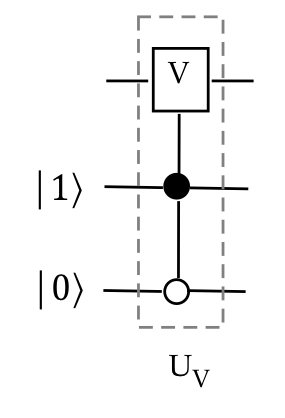
\includegraphics[width=2in]{notes/figs/n09/18multicontrol3.png}
        \caption{$U_V$}
        \label{fig:18multicontrol3}
    \end{figure}
    
    Here, when the 2nd and 3rd qubits are in $|10\rangle$, the $V$ gate is applied. Thus, the only two 3-qubit vectors that will activate $V$ are the adjacent states $|010\rangle$ and $|110\rangle$. Suppose the 3-qubit unitary $U_{V}$ describes the controlled gate above. Then, for any linear combination of $|010\rangle$ and $|110\rangle$
    
    $$
    \begin{aligned}
    U_{V}(p|010\rangle+q|110\rangle) &=p V|0\rangle|10\rangle+q V|1\rangle|10\rangle \\
    &=p(a|0\rangle+c|1\rangle)|10\rangle+q(b|0\rangle+d|1\rangle)|10\rangle \\
    &=(a p+b q)|0\rangle|10\rangle+(b p+d q)|1\rangle|10\rangle \\
    &=(a p+b q)|010\rangle+(b p+d q)|110\rangle
    \end{aligned}
    $$
    
    This suggests that we can make the desired two-level-unitary action work for adjacent vectors. To make it work for our original pair $|001\rangle$ and $|110\rangle$, we form a "word ladder" to go from $|001\rangle$ to $|010\rangle$:
    
    $$
    001 \rightarrow 000 \rightarrow 010
    $$
    
    which is adjacent to $|110\rangle$. We already know how to do vector conversions where two successive vectors different by a bit in the binary representation. Let's draw the circuit for this example shown in Figure \ref{fig:19multicontrol4}.
    
    \begin{figure}
        \centering
        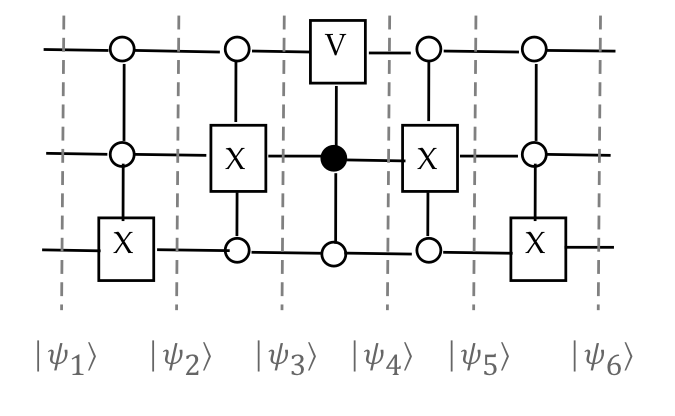
\includegraphics[width=4in]{notes/figs/n09/19multicontrol4.png}
        \caption{word ladder}
        \label{fig:19multicontrol4}
    \end{figure}
    
    Then for
    
    $$
    \left|\psi_{1}\right\rangle=p|001\rangle+q|110\rangle
    $$
    
    we get
    
    $$
    \begin{aligned}
    &\left|\psi_{2}\right\rangle=p|000\rangle+q|110\rangle \\
    &\left|\psi_{3}\right\rangle=p|010\rangle+q|110\rangle \\
    &\left|\psi_{4}\right\rangle=(a p+b q)|010\rangle+(b p+d q)|110\rangle \\
    &\left|\psi_{5}\right\rangle=(a p+b q)|000\rangle+(b p+d q)|110\rangle \\
    &\left|\psi_{6}\right\rangle=(a p+b q)|001\rangle+(b p+d q)|110\rangle
    \end{aligned}
    $$
    
    The latter two return the transformed state $|010\rangle$ back to the original $|001\rangle$. The same circuit does nothing to the other standard-basis vectors. Each of the above multiply-controlled 1-qubit operation can be decomposed into 1-qubit standard gates and $C_{N o T}$ gates. So, finally, we have a circuit for an arbitrary two-level matrix. Let's state this as a theorem: Theorem 7.1: An arbitrary n-qubit unitary can be constructed out of 1-qubit standard gates and $C_{NOT}$ gates. How many gates? Unfortunately, the decomposition we've described needs an exponential number of gates. Consider the breakdown into two-level unitaries: The starting point is a $N \times N=2^{n} \times 2^{n}$ matrix. It takes $N-1$ steps to create zeroes in the first column (and row). Then, $N-2$ for the second column, and so on. Thus, overall: $N-1+N-2+\ldots+1=N(N-1) / 2$ two-level unitaries. This is approximately of the order of $N^{2}=2^{2 n}$. This is already exponential (in the number of qubits). The staging of each two-level unitary is linear, because at most 1-bit "word ladder" changes are needed for any two-level unitary. Thus, while theoretically interesting, it is not a practical approach. Theoretical results about approximation: One might ask: is it possible to approximate a unitary with circuit that has a polynomial number of gates? Unfortunately, the answer is no. For any given set of gates, one can construct qubit states that will need an exponential number of gates to construct from the all- 0 state. Of course, this says little about the types of unitaries that tend to appear in well-known algorithms. A related approximation result: the famous Solovay-Kitaev theorem. This is about 1-qubit unitaries. Recall: we showed how to use K, R, T gates to construct any unitary. However, the parameters of these gates were determined by solving equations. What if your hardware had only a fixed set of gates with fixed parameters? The S-K theorem shows that, nonetheless, it's possibly to efficiently approximate any 1-qubit unitary with a polynomial number of gates from a fixed set.
    
    
\end{document}